\documentclass[11pt]{article}
\usepackage{mathblatt}


\begin{document}
\pfheftstil
\pfheftkopf{Pythagoras: Seite berechnen}{P10}
\pfrueckblick
\begin{pfaufg}{}{1.}{}
Berechne: 6² + 8²; √100; 13² $-$ 5²; √144.
\rechenplatz{1}
\fusshilfe{\mbox{1:~100; 10; 144; 12}}
\end{pfaufg}
\begin{pfaufg}{}{2.}{}
Kreuze an, wo immer ein rechter Winkel ist: zwischen Höhe und Radius eines Kegels; zwischen den Diagonalen eines Drachenvierecks; zwischen zwei Seiten eines Parallelogramms.
\fusshilfe{\mbox{2:~ja; ja; nein}}
\end{pfaufg}
\pfstufekopf[skatheteoderhypotenus]{Kathete oder Hypotenuse direkt}{in 3 der letzten 5 Prüfungen}
\pfgruppe{erst verstehen – nicht rechnen}
\begin{pfaufg}{}{3.}{}
Kreise im Dreieck den rechten Winkel ein. Beschrifte die Hypotenuse mit H. Wie lang ist die Hypotenuse?
\par\smallskip\noindent \dreieckrw{5}{1.12}{$40$ cm}{$9$ cm}{$41$ cm}\par
\par\noindent \leerfeld[cm] \par
\fusshilfe{\mbox{3:~Hypotenuse: $41$ cm}}
\end{pfaufg}
\begin{pfaufg}{}{4.}{}
Gilt für das Dreieck in der Figur der Satz des Pythagoras? \janein
\par\smallskip\noindent \dreieckrw{5}{3.57}{}{}{}\par
\fusshilfe{\mbox{4:~rechter Winkel bei C}}
\end{pfaufg}
\par\addvspace{4pt}{\small\uebersichtskasten{\textbf{Merke:} Die Hypotenuse liegt dem rechten Winkel gegenüber und ist die längste Seite; die beiden anderen sind Katheten. Der Satz spricht über Flächen (Quadrate über den Seiten), nicht über Längen. Merkregel: Hypotenuse gesucht $\to$ plus, Kathete gesucht $\to$ minus.}}\par
\pfgruppe{}
\begin{pfaufg}{}{5.}{}
In einem rechtwinkligen Dreieck sind die Katheten $a = 36$ cm und $b = 15$ cm lang. Berechne die Länge der Hypotenuse $c$.
\par\noindent c² = \leerfeld , c = \leerfeld[cm] \par
\fusshilfe{\mbox{5:~$c = 39$ cm}}
\end{pfaufg}
\begin{pfaufg}{}{6.}{}
Im Dreieck ist eine Seite mit ? markiert. Wie lang ist diese Seite?
\par\smallskip\noindent \dreieck{(0,0)}{(5,0)}{(1.4,2.24)}{45\text{ cm}}{28\text{ cm}}{?}{}{}{90^\circ}\par
\par\noindent \leerfeld[cm] \par
\fusshilfe{\mbox{6:~2\,809, Seite; $53$ cm}}
\end{pfaufg}
\begin{pfaufg}{}{7.}{}
In einem rechtwinkligen Dreieck sind $a = 4$ cm und $b = 9$ cm die Katheten. Berechne die Länge der Hypotenuse $c$. Runde auf eine Stelle nach dem Komma.
\par\noindent c² = \leerfeld , c $\approx$ \leerfeld[cm] \par
\fusshilfe{\mbox{7:~$\sqrt{97} \approx 9{,}8$ cm}}
\end{pfaufg}
\begin{pfaufg}{}{8.}{}
In einem rechtwinkligen Dreieck sind $a = 1{,}2$ m und $b = 50$ cm die Katheten. Berechne die Länge der Hypotenuse $c$ in cm.
\par\noindent c = \leerfeld[cm] \par
\fusshilfe{\mbox{8:~$130$ cm}}
\end{pfaufg}
\begin{pfaufg}{}{9.}{}
Leiterlänge und Abstand des Leiterfußes zur Wand sind gegeben, gesucht ist die Höhe an der Wand. Plus oder minus? 
\pfkreuzzeile{Hypotenuse gesucht – plus}\pfkreuzzeile{Kathete gesucht – minus}
\fusshilfe{\mbox{9:~minus}}
\end{pfaufg}
\begin{pfaufg}{}{10.}{}
In einem rechtwinkligen Dreieck ist die Hypotenuse $c = 85$ cm lang. Eine Kathete ist $b = 13$ cm lang. Berechne die Länge der Kathete $a$.
\par\noindent a² = \leerfeld , a = \leerfeld[cm] \par
\fusshilfe{\mbox{10:~$a = 84$ cm}}
\end{pfaufg}
\pfgruppe{}
\begin{pfaufg}{nach P10 ’24}{11.}{}
In einem rechtwinkligen Dreieck ist die Hypotenuse 10 cm und eine Kathete 8 cm lang. Berechne die andere Kathete.
\rechenplatz{1}
\fusshilfe{\mbox{11:~√(10² $-$ 8²) = √36 = 6 cm}}
\end{pfaufg}
\pfgruppe{}
\begin{pfaufg}{}{12.}{}
Kreuze an, welche Aussage im rechtwinkligen Dreieck gilt. 
\pfkreuzzeile{Die Hypotenuse ist die kürzeste Seite.}\pfkreuzzeile{Das Quadrat über der Hypotenuse ist so groß wie die zwei Quadrate über den Katheten zusammen.}\pfkreuzzeile{Die zwei Katheten sind zusammen so lang wie die Hypotenuse.}
\end{pfaufg}
\pfgruppe{}
\begin{pfaufg}{nach P10 ’15}{13.}{}
Ein rechtwinkliges Dreieck hat die Katheten 0,68 m und 0,40 m. Berechne die Länge der Hypotenuse.
\rechenplatz{1}
\fusshilfe{\mbox{13:~h\_s = √(0,68² + 0,40²) = √0,6224 $\approx$ 0,79 m}}
\end{pfaufg}
\begin{pfaufg}{nach P10 ’25}{14.}{}
Ein rechtwinkliges Dreieck hat die Katheten 3 cm und 6 cm. Berechne die Hypotenuse.
\rechenplatz{1}
\fusshilfe{\mbox{14:~√(3² + 6²) = √45 = 3√5 cm $\approx$ 6,71 cm}}
\end{pfaufg}
\pfgruppe{}
\begin{pfaufg}{P10 ’20}{15.}{}
Im Dreieck ABC ist bei C ein rechter Winkel. Die Strecke BC ist 12 m lang, die Strecke AC 34 m. Berechne die Länge der Strecke AB.
\par\smallskip\noindent \begin{tikzpicture}[x=1.000cm,y=1.000cm,line width=0.6pt,baseline=(current bounding box.north)]\draw (0.000,3.500) -- (6.000,3.500) -- (0.000,0.000) -- cycle;\draw[dashed] (0.000,2.800) -- (6.000,3.500);\draw[line width=0.4pt] (0.000,3.220) -- (0.280,3.220) -- (0.280,3.500);\fill (0.140,3.360) circle (0.6pt);\node[font=\small,inner sep=1pt] at (-0.259,3.651) {$C$};\node[font=\small,inner sep=1pt] at (6.288,3.584) {$B$};\node[font=\small,inner sep=1pt] at (-0.195,-0.228) {$A$};\node[font=\small,inner sep=1pt] at (-0.292,2.868) {$Q$};\fill (0.000,2.800) circle (1.4pt);\node[font=\scriptsize,mbgrau,anchor=north west] at ([yshift=-2pt]current bounding box.south west) {nicht maßstabsgerecht};\end{tikzpicture}\par
\rechenplatz{2}
\fusshilfe{\mbox{15:~AB = 10√13 $\approx$ 36,1 m}}
\end{pfaufg}
\begin{pfaufg}{P10 ’16}{16.}{}
An einem Fluss liegen der Bioladen C, eine Brücke D und eine Anlegestelle B auf einer Geraden am Ufer, in dieser Reihenfolge. Von einem Ausflugslokal A führt ein 920 m langer Weg zum Bioladen; vom Bioladen bis zur Brücke sind es 541 m. Die Strecke AD steht senkrecht auf dem Ufer. Am Bioladen ist der Winkel zwischen den Wegen nach A und nach D 54° groß, am Lokal der Winkel zwischen den Richtungen nach C und nach B 70°. Vom Lokal A soll ein neuer Weg direkt zur Brücke D führen. Ermittle die Länge von AD.
\par\smallskip\noindent \begin{tikzpicture}[line width=0.6pt,baseline=(current bounding box.north)]\draw (-0.6,3.12) -- (6.4,1.72);\draw (2.49,-0.15) -- (0.00,3.00);\draw (2.49,-0.15) -- (5.60,1.88);\draw[dashed] (2.49,-0.15) -- (3.00,2.40);\node[font=\small,anchor=south] at (0.00,3.00) {$C$};\node[font=\small,anchor=south] at (3.00,2.40) {$D$};\node[font=\small,anchor=south] at (5.60,1.88) {$B$};\node[font=\small,anchor=north] at (2.49,-0.15) {$A$};\path (2.49,-0.15) -- node[font=\scriptsize,left] {920 m} (0.00,3.00);\path (0.00,3.00) -- node[font=\scriptsize,above] {541 m} (3.00,2.40);\draw[line width=0.4pt] (0.00,3.00) ++(308.33096706931855:0.55) arc (308.33096706931855:348.69006752597977:0.55);\node[font=\scriptsize,fill=white,inner sep=0.5pt] at ($(0.00,3.00)+(328.51051729764913:0.8500000000000001)$) {54°};\draw[line width=0.4pt] (2.49,-0.15) ++(33.128308197129584:0.7) arc (33.128308197129584:128.33096706931855:0.7);\node[font=\scriptsize,fill=white,inner sep=0.5pt] at ($(2.49,-0.15)+(80.72963763322406:1.0)$) {70°};\draw[line width=0.4pt] (2.95,2.15) -- (3.20,2.11) -- (3.25,2.35);\node[font=\scriptsize,mbgrau,anchor=west] at (6.4,1.72) {Ufer};\node[font=\scriptsize,mbgrau,anchor=north west] at ([yshift=-2pt]current bounding box.south west) {nicht maßstabsgerecht};\end{tikzpicture}\par
\rechenplatz{2}
\fusshilfe{\mbox{16:~AD = √553 719 $\approx$ 744 m}}
\end{pfaufg}
\par\addvspace{4pt}\Needspace*{0.3\textheight}\begin{list}{}{\setlength{\leftmargin}{8mm}\setlength{\topsep}{0pt}}\item[]
\noindent{\footnotesize\color{mbgrau}gleiche Art \textperiodcentered{} 4$\times$ geprüft – kannst du überspringen}\par
\begin{pfaufg}{P10 ’19}{17.}{}
Beim Fußballtraining spielen sich drei Kinder den Ball zu: Amir steht bei A, Ben bei B, Chris bei C. Zwischen Ben und Amir sind es 4 m, zwischen Amir und Chris 9 m. Bei B ist ein rechter Winkel; der Winkel bei A heißt $\alpha$. Ermittle den Abstand zwischen Ben und Chris.\par\smallskip\noindent \begin{tikzpicture}[x=1.000cm,y=1.000cm,line width=0.6pt,baseline=(current bounding box.north)]\draw (0.000,0.000) -- (0.000,3.500) -- (6.000,0.000) -- cycle;\draw[line width=0.4pt] (0.280,0.000) -- (0.280,0.280) -- (0.000,0.280);\fill (0.140,0.140) circle (0.6pt);\draw[line width=0.4pt] (0.000,3.080) arc (-90.00:-30.26:0.420);\node[font=\scriptsize,inner sep=0.5pt,fill=white] at (0.369,2.858) {$\alpha$};\node[font=\scriptsize,anchor=east,inner sep=2pt] at (0.000,1.750) {4 m};\node[font=\scriptsize,anchor=south,inner sep=2pt] at (3.000,1.750) {9 m};\node[font=\small,inner sep=1pt] at (-0.259,-0.151) {$B$};\node[font=\small,inner sep=1pt] at (-0.195,3.728) {$A$};\node[font=\small,inner sep=1pt] at (6.288,-0.084) {$C$};\node[font=\scriptsize,mbgrau,anchor=north west] at ([yshift=-2pt]current bounding box.south west) {nicht maßstabsgerecht};\end{tikzpicture}\par\par\vspace{7mm}\noindent{\color{black!45}\rule{\linewidth}{0.4pt}}
\fusshilfe{\mbox{17:~BC = √65 $\approx$ 8,06 m}}
\end{pfaufg}
\begin{pfaufg}{P10 ’24}{18.}{}
Eine Seilbahn führt vom Ort B im Tal zum Ort A auf einem Berg. F liegt senkrecht unter A auf der Höhe von B; bei F ist ein rechter Winkel. FB ist 255 m lang, die Seilbahnstrecke AB 384 m. Eine zweite Seilbahn verbindet B mit dem Ort C auf einem anderen Berg. Bei B heißt der Winkel zwischen BF und BA $\beta_1$, der Winkel zwischen BA und BC $\beta_2$; bei A heißt der Winkel zwischen AB und AC $\alpha$. Die Strecke FA ist der Höhenunterschied zwischen B und A. Berechne diesen Höhenunterschied.\par\smallskip\noindent \begin{tikzpicture}[x=1.000cm,y=1.000cm,line width=0.6pt,baseline=(current bounding box.north)]\draw (0.000,3.500) -- (0.000,0.000) -- (6.000,0.000) -- cycle;\draw[] (6.000,3.500) -- (0.000,3.500);\draw[] (6.000,3.500) -- (6.000,0.000);\draw[line width=0.4pt] (0.280,0.000) -- (0.280,0.280) -- (0.000,0.280);\fill (0.140,0.140) circle (0.6pt);\draw[line width=0.4pt] (5.352,0.378) arc (149.74:180.00:0.750);\node[font=\scriptsize,inner sep=0.5pt,fill=white] at (4.967,0.279) {$\beta_1$};\draw[line width=0.4pt] (6.000,0.420) arc (90.00:149.74:0.420);\node[font=\scriptsize,inner sep=0.5pt,fill=white] at (5.631,0.642) {$\beta_2$};\draw[line width=0.4pt] (0.000,3.080) arc (-90.00:-30.26:0.420);\node[font=\scriptsize,inner sep=0.5pt,fill=white] at (0.369,2.858) {$\alpha$};\node[font=\scriptsize,anchor=north,inner sep=2pt] at (3.000,0.000) {255 m};\node[font=\scriptsize,anchor=south,inner sep=2pt] at (3.000,1.750) {384 m};\node[font=\small,inner sep=1pt] at (-0.195,3.728) {$A$};\node[font=\small,inner sep=1pt] at (6.259,3.651) {$C$};\node[font=\small,inner sep=1pt] at (-0.259,-0.151) {$F$};\node[font=\small,inner sep=1pt] at (6.288,-0.084) {$B$};\node[font=\scriptsize,mbgrau,anchor=north west] at ([yshift=-2pt]current bounding box.south west) {nicht maßstabsgerecht};\end{tikzpicture}\par\par\vspace{7mm}\noindent{\color{black!45}\rule{\linewidth}{0.4pt}}
\fusshilfe{\mbox{18:~FA = 3√9159 $\approx$ 287,1 m}}
\end{pfaufg}
\begin{pfaufg}{P10 ’26}{19.}{}
Im Viereck ABCD sind gegenüberliegende Seiten parallel. Die Seite BC ist 32 cm lang. Die Seite AB wird über B hinaus bis F verlängert; BF ist 13 cm lang. Die Höhe h = CF steht senkrecht auf AF. Der Winkel bei B zwischen BF und BC heißt $\varepsilon$. Berechne die Höhe h.\par\smallskip\noindent \begin{tikzpicture}[x=0.714cm,y=0.714cm,line width=0.6pt,baseline=(current bounding box.north)]\draw (0.000,0.000) -- (6.000,0.000) -- (8.400,3.500) -- (2.400,3.500) -- cycle;\draw[] (6.000,0.000) -- (8.400,0.000);\draw[dashed] (8.400,3.500) -- (8.400,0.000);\draw[line width=0.4pt] (8.400,0.392) -- (8.008,0.392) -- (8.008,0.000);\fill (8.204,0.196) circle (0.6pt);\draw[line width=0.4pt] (6.588,0.000) arc (0.00:55.56:0.588);\node[font=\scriptsize,inner sep=0.5pt,fill=white] at (6.917,0.483) {$\varepsilon$};\node[font=\scriptsize,anchor=west,inner sep=2pt] at (8.400,1.750) {$h$};\node[font=\scriptsize,anchor=west,inner sep=2pt] at (7.200,1.750) {32 cm};\node[font=\scriptsize,anchor=north,inner sep=2pt] at (7.200,0.000) {13 cm};\node[font=\small,inner sep=1pt] at (-0.388,-0.162) {$A$};\node[font=\small,inner sep=1pt] at (6.301,-0.293) {$B$};\node[font=\small,inner sep=1pt] at (8.788,3.662) {$C$};\node[font=\small,inner sep=1pt] at (2.099,3.793) {$D$};\node[font=\small,inner sep=1pt] at (8.788,-0.162) {$F$};\node[font=\scriptsize,mbgrau,anchor=north west] at ([yshift=-2pt]current bounding box.south west) {nicht maßstabsgerecht};\end{tikzpicture}\par\par\vspace{7mm}\noindent{\color{black!45}\rule{\linewidth}{0.4pt}}
\fusshilfe{\mbox{19:~h = 3√95 $\approx$ 29,2 cm}}
\end{pfaufg}
\end{list}
\pfgruppe{}
\begin{pfaufg}{P10 ’22}{20.}{}
Gegeben ist ein Dreieck ABC, das nicht rechtwinklig ist. Die Höhe $h_c$ von C auf die Seite AB ist etwa 7,4 m lang; ihr Fußpunkt heißt D. Die Seite b = AC ist 14,1 m lang, der Winkel bei B ist 52° groß. Der Winkel bei C zwischen AC und der Höhe heißt $\gamma_1$. Weise nach, dass die Strecke AD etwa 12,0 m lang ist.
\par\smallskip\noindent \begin{tikzpicture}[x=1.000cm,y=1.000cm,line width=0.6pt,baseline=(current bounding box.north)]\draw (0.000,0.000) -- (6.000,0.000) -- (3.000,3.500) -- cycle;\draw[dashed] (3.000,3.500) -- (3.000,0.000);\draw[line width=0.4pt] (3.000,0.280) -- (2.720,0.280) -- (2.720,0.000);\fill (2.860,0.140) circle (0.6pt);\draw[line width=0.4pt] (0.420,0.000) arc (0.00:49.40:0.420);\node[font=\scriptsize,inner sep=0.5pt,fill=white] at (0.672,0.309) {$\alpha$};\draw[line width=0.4pt] (5.727,0.319) arc (130.60:180.00:0.420);\node[font=\scriptsize,inner sep=0.5pt,fill=white] at (5.164,0.384) {52°};\draw[line width=0.4pt] (3.000,3.080) arc (-90.00:0.00:0.420);\node[font=\scriptsize,inner sep=0.5pt,fill=white] at (3.523,2.977) {$\gamma_1$};\node[font=\scriptsize,anchor=west,inner sep=2pt] at (3.000,1.750) {$h_c$};\node[font=\scriptsize,anchor=east,inner sep=2pt] at (1.500,1.750) {b = 14,1 m};\node[font=\scriptsize,anchor=west,inner sep=2pt] at (4.500,1.750) {a};\node[font=\small,inner sep=1pt] at (-0.280,-0.109) {$A$};\node[font=\small,inner sep=1pt] at (6.280,-0.109) {$B$};\node[font=\small,inner sep=1pt] at (3.000,3.800) {$C$};\node[font=\small,inner sep=1pt] at (3.000,-0.300) {$D$};\node[font=\scriptsize,mbgrau,anchor=north west] at ([yshift=-2pt]current bounding box.south west) {nicht maßstabsgerecht};\end{tikzpicture}\par
\rechenplatz{2}
\fusshilfe{\mbox{20:~AD = √(14,1² $-$ 7,4²) $\approx$ 12,0 m}}
\end{pfaufg}
\pfgruppe{}
\begin{pfaufg}{P10 ’22}{\llap{\textasteriskcentered\,}21.}{}
Ein Becher hat die Form eines Zylinders ohne Deckel. Er ist h = 7 cm hoch und hat den Radius r = 3,2 cm. Ein Becher hat die Form eines Zylinders ohne Deckel; er ist 7 cm hoch und hat den Radius 3,2 cm. Ein Rührstab steht schräg im Becher: Er berührt unten den Rand des Bodens und lehnt oben am gegenüberliegenden Rand. 2 cm des Stabs ragen über den Becher hinaus. Bestimme die Länge des Stabs.
\par\smallskip\noindent \begin{tikzpicture}[line width=0.6pt,baseline=(current bounding box.north)]\draw (-1.10,0.00) arc (180:360:1.10 and 0.33);\draw[dashed] (1.10,0.00) arc (0:180:1.10 and 0.33);\draw (-1.1,0) -- (-1.1,2.4); \draw (1.1,0) -- (1.1,2.4);\draw (0,2.4) ellipse (1.1 and 0.33);\draw[line width=1.6pt] (-0.99,-0.15) -- (1.38,3.15);\node[font=\scriptsize,mbgrau,anchor=north west] at ([yshift=-2pt]current bounding box.south west) {nicht maßstabsgerecht};\end{tikzpicture}\par
\rechenplatz{3}
\fusshilfe{\mbox{21:~√89,96 + 2 $\approx$ 11,5 cm}}
\end{pfaufg}
\pfstufekopf[sgleichungaufstellen]{Gleichung aufstellen}{in 3 der letzten 5 Prüfungen}
\pfgruppe{}
\begin{pfaufg}{P10 ’22}{22.}{}
Kreuze die Aussage an, die für jedes rechtwinklige Dreieck stimmt:
\pfkreuzzeile{Die Seite gegenüber dem rechten Winkel ist eine Kathete.}\pfkreuzzeile{$c=a+b$}\pfkreuzzeile{Die beiden Kathetenquadrate haben zusammen denselben Flächeninhalt wie das Hypotenusenquadrat}
\end{pfaufg}
\begin{pfaufg}{P10 ’17}{23.}{}
Im abgebildeten Dreieck sind x und y die Katheten, z ist die Hypotenuse. Kreuze die Gleichung an, die für dieses Dreieck gilt:
\pfkreuzzeile{$x^2=y^2+z^2$}\pfkreuzzeile{$z^2=x^2-y^2$}\pfkreuzzeile{$z^2\cdot y^2=x^2$}\pfkreuzzeile{$z^2=x^2+y^2$}
\par\smallskip\noindent 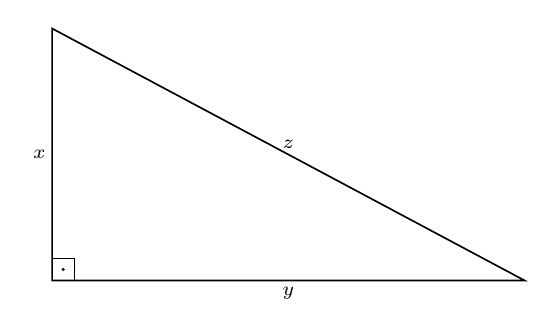
\begin{tikzpicture}[x=1.000cm,y=1.000cm,line width=0.6pt,baseline=(current bounding box.north)]\draw (0.000,0.000) -- (6.000,0.000) -- (0.000,3.200) -- cycle;\draw[line width=0.4pt] (0.280,0.000) -- (0.280,0.280) -- (0.000,0.280);\fill (0.140,0.140) circle (0.6pt);\node[font=\scriptsize,anchor=east,inner sep=2pt] at (0.000,1.600) {$x$};\node[font=\scriptsize,anchor=north,inner sep=2pt] at (3.000,0.000) {$y$};\node[font=\scriptsize,anchor=south,inner sep=2pt] at (3.000,1.600) {$z$};\end{tikzpicture}\par
\fusshilfe{\mbox{23:~z² = x² + y²}}
\end{pfaufg}
\par\addvspace{4pt}\Needspace*{0.3\textheight}\begin{list}{}{\setlength{\leftmargin}{8mm}\setlength{\topsep}{0pt}}\item[]
\noindent{\footnotesize\color{mbgrau}gleiche Art \textperiodcentered{} 3$\times$ geprüft – kannst du überspringen}\par
\begin{pfaufg}{P10 ’21}{24.}{}
Im abgebildeten Dreieck sind x und y die Katheten, z ist die Hypotenuse. Kreuze die Formel an, mit der man z berechnet:\pfkreuzzeile{$z=\sqrt{x^2-y^2}$}\pfkreuzzeile{$z=\sqrt{x^2+y^2}$}\pfkreuzzeile{$z=\sqrt{y^2-x^2}$}\pfkreuzzeile{$z=y^2+x^2$}\par\smallskip\noindent 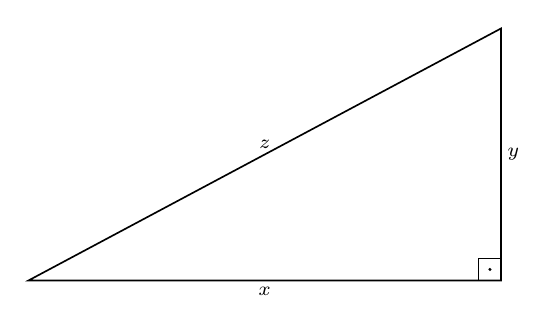
\begin{tikzpicture}[x=1.000cm,y=1.000cm,line width=0.6pt,baseline=(current bounding box.north)]\draw (6.000,0.000) -- (0.000,0.000) -- (6.000,3.200) -- cycle;\draw[line width=0.4pt] (6.000,0.280) -- (5.720,0.280) -- (5.720,0.000);\fill (5.860,0.140) circle (0.6pt);\node[font=\scriptsize,anchor=north,inner sep=2pt] at (3.000,0.000) {$x$};\node[font=\scriptsize,anchor=west,inner sep=2pt] at (6.000,1.600) {$y$};\node[font=\scriptsize,anchor=south,inner sep=2pt] at (3.000,1.600) {$z$};\end{tikzpicture}\par
\fusshilfe{\mbox{24:~z = √(x² + y²)}}
\end{pfaufg}
\begin{pfaufg}{P10 ’24}{25.}{}
Im abgebildeten Dreieck sind y und z die Katheten, x ist die Hypotenuse. Kreuze die Gleichung an, mit der man die Länge von z berechnen kann:\pfkreuzzeile{$z=x^2-y^2$}\pfkreuzzeile{$z=\sqrt{x^2+y^2}$}\pfkreuzzeile{$z=x+y$}\pfkreuzzeile{$z=\sqrt{x^2-y^2}$}\par\smallskip\noindent 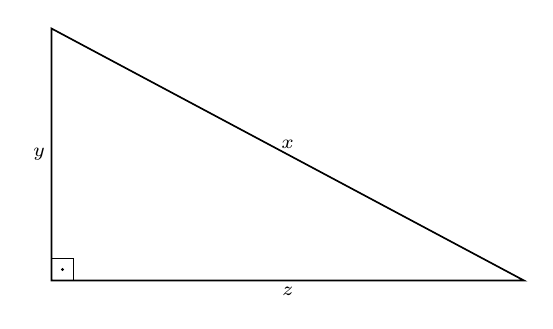
\begin{tikzpicture}[x=1.000cm,y=1.000cm,line width=0.6pt,baseline=(current bounding box.north)]\draw (0.000,0.000) -- (6.000,0.000) -- (0.000,3.200) -- cycle;\draw[line width=0.4pt] (0.280,0.000) -- (0.280,0.280) -- (0.000,0.280);\fill (0.140,0.140) circle (0.6pt);\node[font=\scriptsize,anchor=east,inner sep=2pt] at (0.000,1.600) {$y$};\node[font=\scriptsize,anchor=north,inner sep=2pt] at (3.000,0.000) {$z$};\node[font=\scriptsize,anchor=south,inner sep=2pt] at (3.000,1.600) {$x$};\end{tikzpicture}\par
\fusshilfe{\mbox{25:~z = √(x² $-$ y²) (vierte Option)}}
\end{pfaufg}
\end{list}
\pfgruppe{}
\begin{pfaufg}{P10 ’26}{26.}{}
Im abgebildeten Dreieck sind u und v die Katheten, w ist die Hypotenuse. Kreuze an, mit welcher Gleichung man w berechnen kann:
\pfkreuzzeile{$w=\sqrt{v^2-u^2}$}\pfkreuzzeile{$w=\sqrt{u^2-v^2}$}\pfkreuzzeile{$w=\sqrt{u^2+v^2}$}
\par\smallskip\noindent 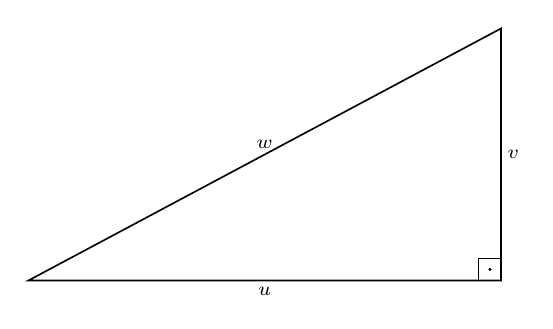
\begin{tikzpicture}[x=1.000cm,y=1.000cm,line width=0.6pt,baseline=(current bounding box.north)]\draw (6.000,0.000) -- (0.000,0.000) -- (6.000,3.200) -- cycle;\draw[line width=0.4pt] (6.000,0.280) -- (5.720,0.280) -- (5.720,0.000);\fill (5.860,0.140) circle (0.6pt);\node[font=\scriptsize,anchor=north,inner sep=2pt] at (3.000,0.000) {$u$};\node[font=\scriptsize,anchor=west,inner sep=2pt] at (6.000,1.600) {$v$};\node[font=\scriptsize,anchor=south,inner sep=2pt] at (3.000,1.600) {$w$};\end{tikzpicture}\par
\fusshilfe{\mbox{26:~w = √(u² + v²) (dritte Option)}}
\end{pfaufg}
\pfstufekopf[sdreieckerstinfigurod]{Dreieck erst in Figur oder Körper finden}{in 2 der letzten 5 Prüfungen}
\pfgruppe{}
\begin{pfaufg}{}{27.}{}
Die Figur zeigt ein gleichschenkliges Trapez mit seiner Höhe. Fahre das rechtwinklige Dreieck aus Höhe, Schenkel und Überstand farbig nach. Schreibe dazu, welche Seiten Katheten sind und welche die Hypotenuse ist.
\par\smallskip\noindent \trapez[hoehe=h]{5}{3}{2.5}\par
\rechenplatz{1}
\fusshilfe{\mbox{27:~Katheten: die Höhe und der Überstand}}
\end{pfaufg}
\pfgruppe{}
\begin{pfaufg}{P10 ’18}{\llap{\textasteriskcentered\,}28.}{}
Ein runder Turm mit 6,4 m Durchmesser hat ein Dach in Form eines Kegels. Die Höhe des Daches ist bekannt. Ein Dachbalken läuft von der Spitze bis zum Rand des Daches. Beschreibe, wie man die Länge eines Dachbalkens berechnen kann.
\par\smallskip\noindent \begin{tikzpicture}[line width=0.6pt,baseline=(current bounding box.north)]\draw (-1.20,0.00) arc (180:360:1.20 and 0.36);\draw[dashed] (1.20,0.00) arc (0:180:1.20 and 0.36);\draw (-1.2,0) -- (0,2.4) -- (1.2,0);\draw[-{Stealth[length=2mm]},line width=0.4pt] (1.9,1.9) node[right,font=\scriptsize] {Dachbalken} -- (0.5,1.4);\node[font=\scriptsize,mbgrau,anchor=north west] at ([yshift=-2pt]current bounding box.south west) {nicht maßstabsgerecht};\end{tikzpicture}\par
\rechenplatz{2}
\fusshilfe{\mbox{28:~s = √(3,2² + h²)}}
\end{pfaufg}
\pfgruppe{}
\begin{pfaufg}{nach P10 ’14}{29.}{}
Ein Kegel hat den Radius 154 m und die Mantellinie 193 m. Berechne seine Höhe.
\rechenplatz{1}
\fusshilfe{\mbox{29:~h = √(193² $-$ 154²) = √13 533 $\approx$ 116,3 m}}
\end{pfaufg}
\begin{pfaufg}{nach P10 ’15}{30.}{}
Berechne den Abstand des Punktes R(5 | 2) vom Ursprung O(0 | 0).
\rechenplatz{1}
\fusshilfe{\mbox{30:~OR = √(5² + 2²) = √29 $\approx$ 5,39 LE}}
\end{pfaufg}
\begin{pfaufg}{nach P10 ’15}{31.}{}
Ein kegelförmiger Hut hat den Radius 1,73 cm und die Höhe 3 cm. Berechne die Länge seiner Mantellinie.
\rechenplatz{1}
\fusshilfe{\mbox{31:~s = √(1,73² + 3²) $\approx$ 3,46 cm}}
\end{pfaufg}
\begin{pfaufg}{nach P10 ’19}{32.}{}
Eine quadratische Pyramide hat die Grundkante 4 m und die Höhe 3 m. Berechne die Höhe einer Seitenfläche.
\rechenplatz{1}
\fusshilfe{\mbox{32:~h\_s = √(3² + 2²) = √13 $\approx$ 3,61 m}}
\end{pfaufg}
\begin{pfaufg}{nach P10 ’21}{33.}{}
Ein Kegel hat den Radius 5 cm und die Höhe 15,03 cm. Berechne die Länge seiner Mantellinie.
\rechenplatz{1}
\fusshilfe{\mbox{33:~s = √(5² + 15,03²) $\approx$ 15,84 cm}}
\end{pfaufg}
\pfgruppe{}
\begin{pfaufg}{nach P10 ’17}{34.}{}
Die Diagonalenabschnitte eines Drachenvierecks sind 8,5 m und 7,5 m lang und stehen senkrecht aufeinander. Berechne die Länge der Seite zwischen ihren Enden.
\rechenplatz{1}
\fusshilfe{\mbox{34:~√(8,5² + 7,5²) = √128,5 $\approx$ 11,34 m}}
\end{pfaufg}
\pfgruppe{}
\begin{pfaufg}{NI ’23}{35.}{}
Eine rechteckige Kinoleinwand ist 38 m breit und 22 m hoch. Berechne die Länge der Diagonale x.
\par\smallskip\noindent \fbox{\parbox{0.9\linewidth}{\footnotesize Skizze: Rechteck 38 m × 22 m, Diagonale x; nicht maßstäblich}}\par
\rechenplatz{2}
\fusshilfe{\mbox{35:~x = √(38² + 22²) m $\approx$ 43,91 m}}
\end{pfaufg}
\pfgruppe{}
\begin{pfaufg}{P10 ’26}{\llap{\textasteriskcentered\,}36.}{}
Ein Turm besteht unten aus einem Zylinder, sein Dach ist ein Kegel. Bekannt sind: h = 25,0 m (Höhe des Zylinders), r = 4,7 m (Radius von Zylinder und Kegel) und s = 8,6 m (Mantellinie des Kegels). Ein Turm besteht aus einem Zylinder (Höhe 25,0 m, Radius 4,7 m) mit einem Kegeldach; die Mantellinie des Kegels ist 8,6 m lang, sein Radius ebenfalls 4,7 m. Bestimme die Gesamthöhe des Turms.
\par\smallskip\noindent \begin{tikzpicture}[line width=0.6pt,baseline=(current bounding box.north)]\draw (-1.00,0.00) arc (180:360:1.00 and 0.30);\draw[dashed] (1.00,0.00) arc (0:180:1.00 and 0.30);\draw (-1.0,0) -- (-1.0,2.6); \draw (1.0,0) -- (1.0,2.6);\draw (-1.00,2.60) arc (180:360:1.00 and 0.30);\draw[dashed] (1.00,2.60) arc (0:180:1.00 and 0.30);\draw (-1.0,2.6) -- (0,3.9000000000000004) -- (1.0,2.6);\draw[dashed] (0,2.6) -- (1.0,2.6);\node[font=\scriptsize,right] at (1.0,1.3) {$h$ = 25,0 m};\node[font=\scriptsize,below,fill=white,inner sep=1pt] at (0.5,2.52) {$r$ = 4,7 m};\node[font=\scriptsize,right] at (0.55,3.35) {$s$ = 8,6 m};\node[font=\scriptsize,mbgrau,anchor=north west] at ([yshift=-2pt]current bounding box.south west) {nicht maßstabsgerecht};\end{tikzpicture}\par
\rechenplatz{3}
\fusshilfe{\mbox{36:~25 + √51,87 $\approx$ 32,2 m}}
\end{pfaufg}
\pfgruppe{}
\begin{pfaufg}{P10 ’25}{37.}{}
Ein Drachenviereck ABCD (A links, D oben, C rechts, B unten) hat die Diagonalen AC = 50 cm und BD = 80 cm. Sie schneiden sich in F im rechten Winkel. Die Strecke DF ist 25 cm lang. Der Winkel bei D heißt $\gamma$. Kreuze an, wie viele Symmetrieachsen das Drachenviereck hat:
\pfkreuzzeile{0}\pfkreuzzeile{1}\pfkreuzzeile{2}\pfkreuzzeile{3}\pfkreuzzeile{4. Bestätige mit einer Rechnung, dass BF 55 cm lang ist. Berechne die Länge der Seite AB}
\par\smallskip\noindent \begin{tikzpicture}[x=1.000cm,y=1.000cm,line width=0.6pt,baseline=(current bounding box.north)]\draw (0.000,1.750) -- (3.000,0.000) -- (6.000,1.750) -- (3.000,3.500) -- cycle;\draw[] (0.000,1.750) -- (3.000,1.750);\draw[] (3.000,1.750) -- (6.000,1.750);\draw[] (3.000,0.000) -- (3.000,1.750);\draw[] (3.000,1.750) -- (3.000,3.500);\draw[line width=0.4pt] (3.000,1.470) -- (3.280,1.470) -- (3.280,1.750);\fill (3.140,1.610) circle (0.6pt);\draw[line width=0.4pt] (2.637,3.288) arc (-149.74:-30.26:0.420);\node[font=\scriptsize,inner sep=0.5pt,fill=white] at (3.000,2.760) {$\gamma$};\node[font=\scriptsize,anchor=west,inner sep=2pt] at (3.000,2.625) {25 cm};\node[font=\small,inner sep=1pt] at (3.000,3.800) {$D$};\node[font=\small,inner sep=1pt] at (3.000,-0.300) {$B$};\node[font=\small,inner sep=1pt] at (-0.300,1.750) {$A$};\node[font=\small,inner sep=1pt] at (6.300,1.750) {$C$};\node[font=\small,inner sep=1pt] at (3.000,1.750) {$F$};\node[font=\scriptsize,mbgrau,anchor=north west] at ([yshift=-2pt]current bounding box.south west) {nicht maßstabsgerecht};\end{tikzpicture}\par
\rechenplatz{3}
\fusshilfe{\mbox{37:~1 Symmetrieachse (BD); 55 cm; 5√146 $\approx$ 60,4 cm}}
\end{pfaufg}
\pfgruppe{}
\begin{pfaufg}{P10 ’25}{38.}{}
Familie Yücel baut an die Stufe vor der Haustür eine feste Rampe für Rollstühle. Die Stufe ist 16 cm hoch; waagerecht ist die Rampe 170 cm lang. Berechne die Länge x der Rampe. Berechne den Anstiegswinkel $\alpha$.
\par\smallskip\noindent \begin{tikzpicture}[line width=0.6pt]\draw (0,0) -- (6,0) -- (6,1.4) -- cycle;\draw (5.7,0) -- (5.7,0.3) -- (6,0.3);\node[below,font=\small] at (3,0) {170 cm};\node[right,font=\small] at (6,0.7) {16 cm};\node[above left,font=\small] at (3,0.7) {$x$};\node[font=\small] at (1.1,0.12) {$\alpha$};\node[font=\scriptsize,mbgrau,anchor=west] at (0,-0.75) {nicht maßstabsgerecht};\end{tikzpicture}\par
\rechenplatz{3}
\fusshilfe{\mbox{38:~x = 2√7289 $\approx$ 170,8 cm; $\alpha$ = tan$^{-1}$($\tfrac{8}{85}$) $\approx$ 5,4°}}
\end{pfaufg}
\pfgruppe{}
\begin{pfaufg}{P10 ’19}{39.}{}
Im Koordinatensystem bilden die Punkte A(0|$-$2), B(2|$-$2) und C(0|2) ein Dreieck. Berechne die Länge der Strecke BC. Berechne die Größe des Winkels $\beta$ bei B.
\par\smallskip\noindent \begin{tikzpicture}\begin{axis}[xmin=-5,xmax=5,ymin=-5,ymax=5,axis lines=middle,tick label style={font=\scriptsize},clip=true,/pgf/number format/use comma,axis line style={-{Stealth[length=2mm]}},every axis plot/.append style={line width=0.9pt},x=0.9cm,y=0.9cm,xtick distance=1,ytick distance=1,enlargelimits=false,grid=both,grid style={mbgitter,line width=0.3pt},major grid style={mbgitter},minor tick num=1,xlabel={$x$},ylabel={$y$},x label style={anchor=west},y label style={anchor=south}]\draw[line width=0.8pt] (axis cs:0,-2) -- (axis cs:2,-2) -- (axis cs:0,2) -- cycle;\fill (axis cs:0,-2) circle (1.6pt) node[above right,font=\small,inner sep=1pt] {$A$};\fill (axis cs:2,-2) circle (1.6pt) node[above right,font=\small,inner sep=1pt] {$B$};\fill (axis cs:0,2) circle (1.6pt) node[above right,font=\small,inner sep=1pt] {$C$};\draw[line width=0.5pt] (axis cs:2,-2) ++(116.5651:0.55cm) arc (116.5651:180:0.55cm);\node[font=\small] at ($(axis cs:2,-2)+(148.2825:0.85cm)$) {$\beta$};\end{axis}\end{tikzpicture}\par
\rechenplatz{4}
\fusshilfe{\mbox{39:~BC = √20 $\approx$ 4,47; $\beta$ = tan$^{-1}$(2) $\approx$ 63,4°}}
\end{pfaufg}
\end{document}